\documentclass[a4paper,12pt]{article}
\usepackage[T1]{fontenc}
\usepackage[utf8]{inputenc}
\usepackage[icelandic]{babel}
\usepackage{graphicx}
\usepackage{subcaption}
\usepackage{hyperref}
\usepackage{biblatex} %Imports biblatex package
\addbibresource{references.bib} %Import the bibliography file

\title{HiDef Textíll: Tæknivæddar prjónavélar og þverfaglegt samstarf}
\author{Helga Ingimundardóttir}
\date{}

\begin{document}

\maketitle

\begin{abstract}
Verkefnið \emph{HiDef Textíll} sameinar hefðbundna textílvinnslu og nútímatækni með
nýsköpun í prjónavélum frá 10. áratugnum. Markmiðið er að snjallvæða úrelda prjónavél
með netsamskiptum og frjálsum hugbúnaði, sem gerir hana að öflugri lausn fyrir
skapandi notkun í dag. Verkefnið byggir á þverfaglegu samstarfi nemenda úr verkfræði,
hagnýttri stærðfræði og fatahönnun og stuðlar að aukinni þátttöku í STEAM-menntun.
Niðurstöður sýna að hægt er að nýta eldri prjónavélar á nýjan hátt og tengja íslenskan
menningararf við stafræna nýsköpun.
\end{abstract}

\section{Inngangur}
Verkefnið \emph{HiDef Textíll} á sér langa sögu og hófst sem persónulegt áhugamál árið
2014, þegar höfundur sá \emph{KnitterStream} \cite{knitterstream} trenda á Twitter.
Þetta var sama vél og amma höfundar átti, Passap E6000 (sjá mynd \ref{fig:skema-e6000}), en hafði setið ónotuð um
áraraðir. Fyrstu tilraunir voru gerðar í FabLab Reykjavík, en verkefnið varð of tímafrekt
á meðan höfundur var enn í doktorsnámi og í fullu starfi. Eftir umræður á kaffistofu VR-II 
eftir að höfundur hóf störf sem akademískur starfsmaður haustið 2023, varð ljóst að hægt 
væri að gera þetta að rannsóknarverkefni. Með styrk frá \emph{Nýsköpunarsjóði námsmanna}
sumarið 2024 tók verkefnið á sig nýja mynd, með fjölmörgum samstarfsaðilum. 
Prjónavélin var til húsa í vélaskála VR-III (sjá mynd \ref{fig:workshop}) við Hjarðarhaga 2 í Reykjavík. Nemendur höfðu einnig aðgang að Sprotamýri, frumkvöðlasetri HÍ í Grósku.

\begin{figure}
    \centering
    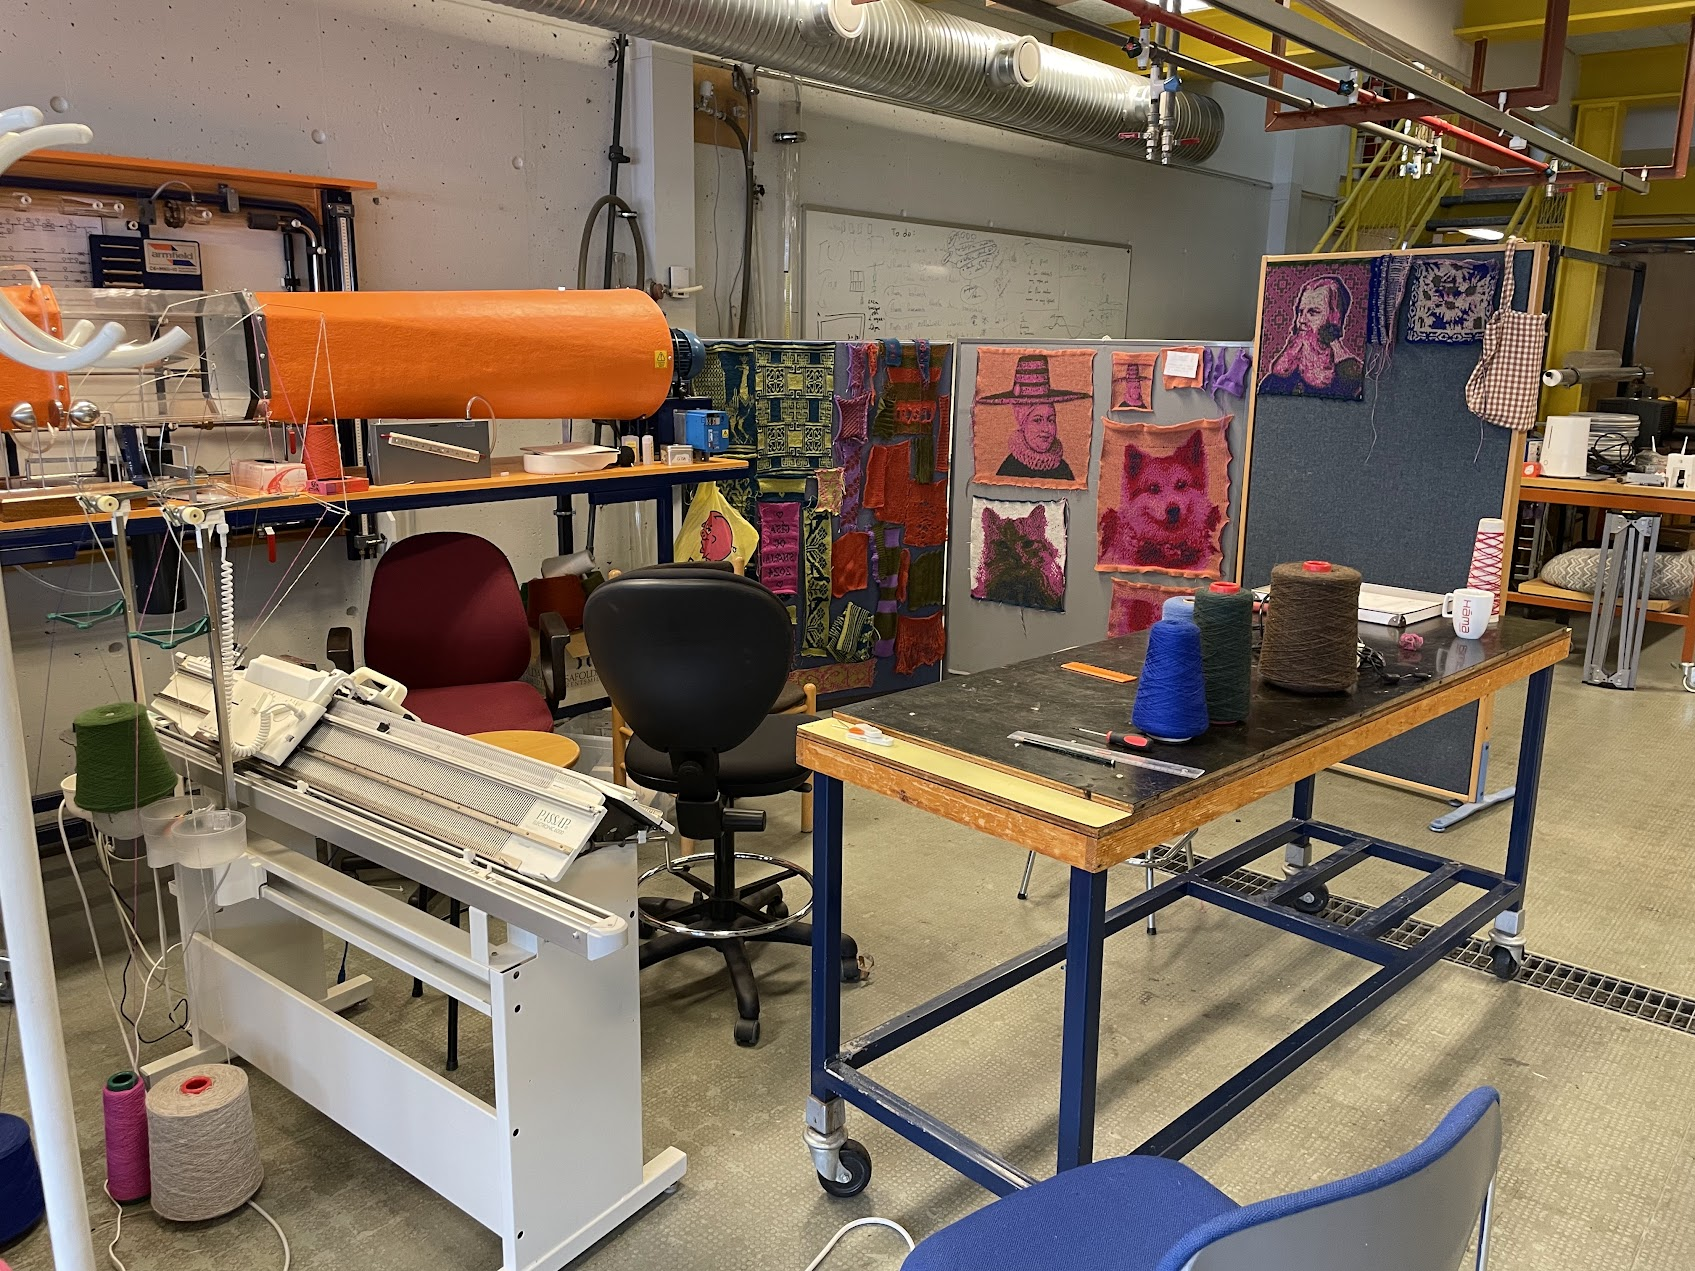
\includegraphics[width=0.8\linewidth]{figs/workshop.jpg}
    \caption{Verkefnið var unnið í vélaskála VR-III.}
    \label{fig:workshop}
\end{figure}


\begin{figure}
    \centering
    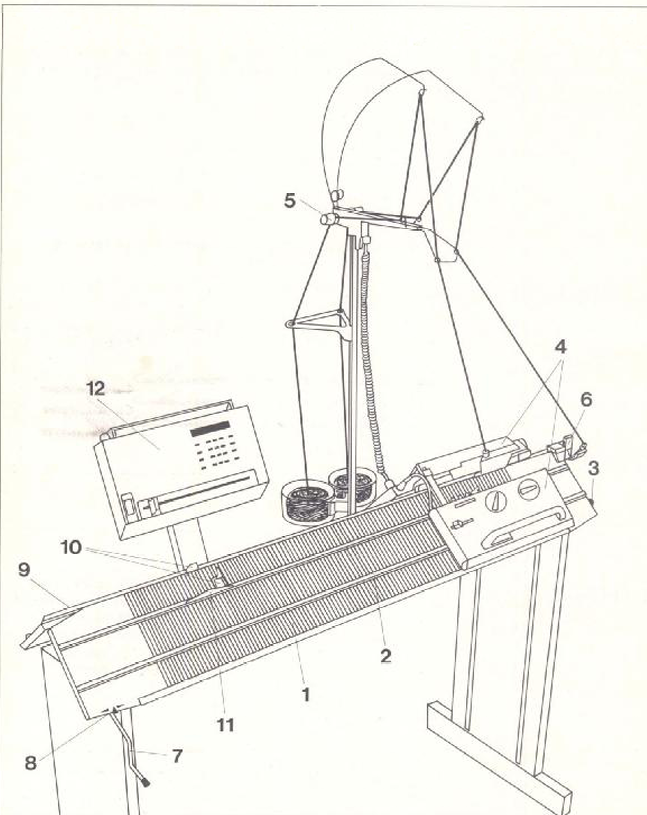
\includegraphics[width=0.4\linewidth]{figs/skema-e6000.png}
    \caption{Tæknileg skýringarmynd af Passap E6000 vélinni.}
    \label{fig:skema-e6000}
\end{figure}

Verkefnið var unnið í samstarfi við Listaháskóla Íslands, frumgerðasmiðju HÍ,
tölvunarfræðideild HÍ, rafmagns- og tölvuverkfræðideild HÍ, Textílmiðstöðina á Blöndósi,
Heimilisiðnaðarfélagið, Þjóðminjasafn Íslands og Marel. Vélin hefur verið sýnd á
Vísindavöku Rannís og UTmessunni hjá Ský, og sótt er um áframhaldandi styrki til að
þróa hana áfram.

\section{Vélrænar uppfærslur}
Til að uppfæra vélbúnað vélarinnar var upprunalega \emph{Form} tölvan (sjá hluta 12 á mynd \ref{fig:skema-e6000}) sem stýrði henni
skipt út fyrir \emph{Arduino} örtölvu (sjá mynd \ref{fig:arduino}). Elías Lúðvíksson, BS nemi í vélaverkfræði við HÍ,
sá um þessa uppfærslu. Eldri tölvukerfið, sem notaðist við DIN-6 snúru og lokuð
hugbúnaðarstýringarkerfi, var fjarlægt og í staðinn var sett inn nýtt kerfi byggt á
opnum hugbúnaði.

\begin{figure}
    \centering
    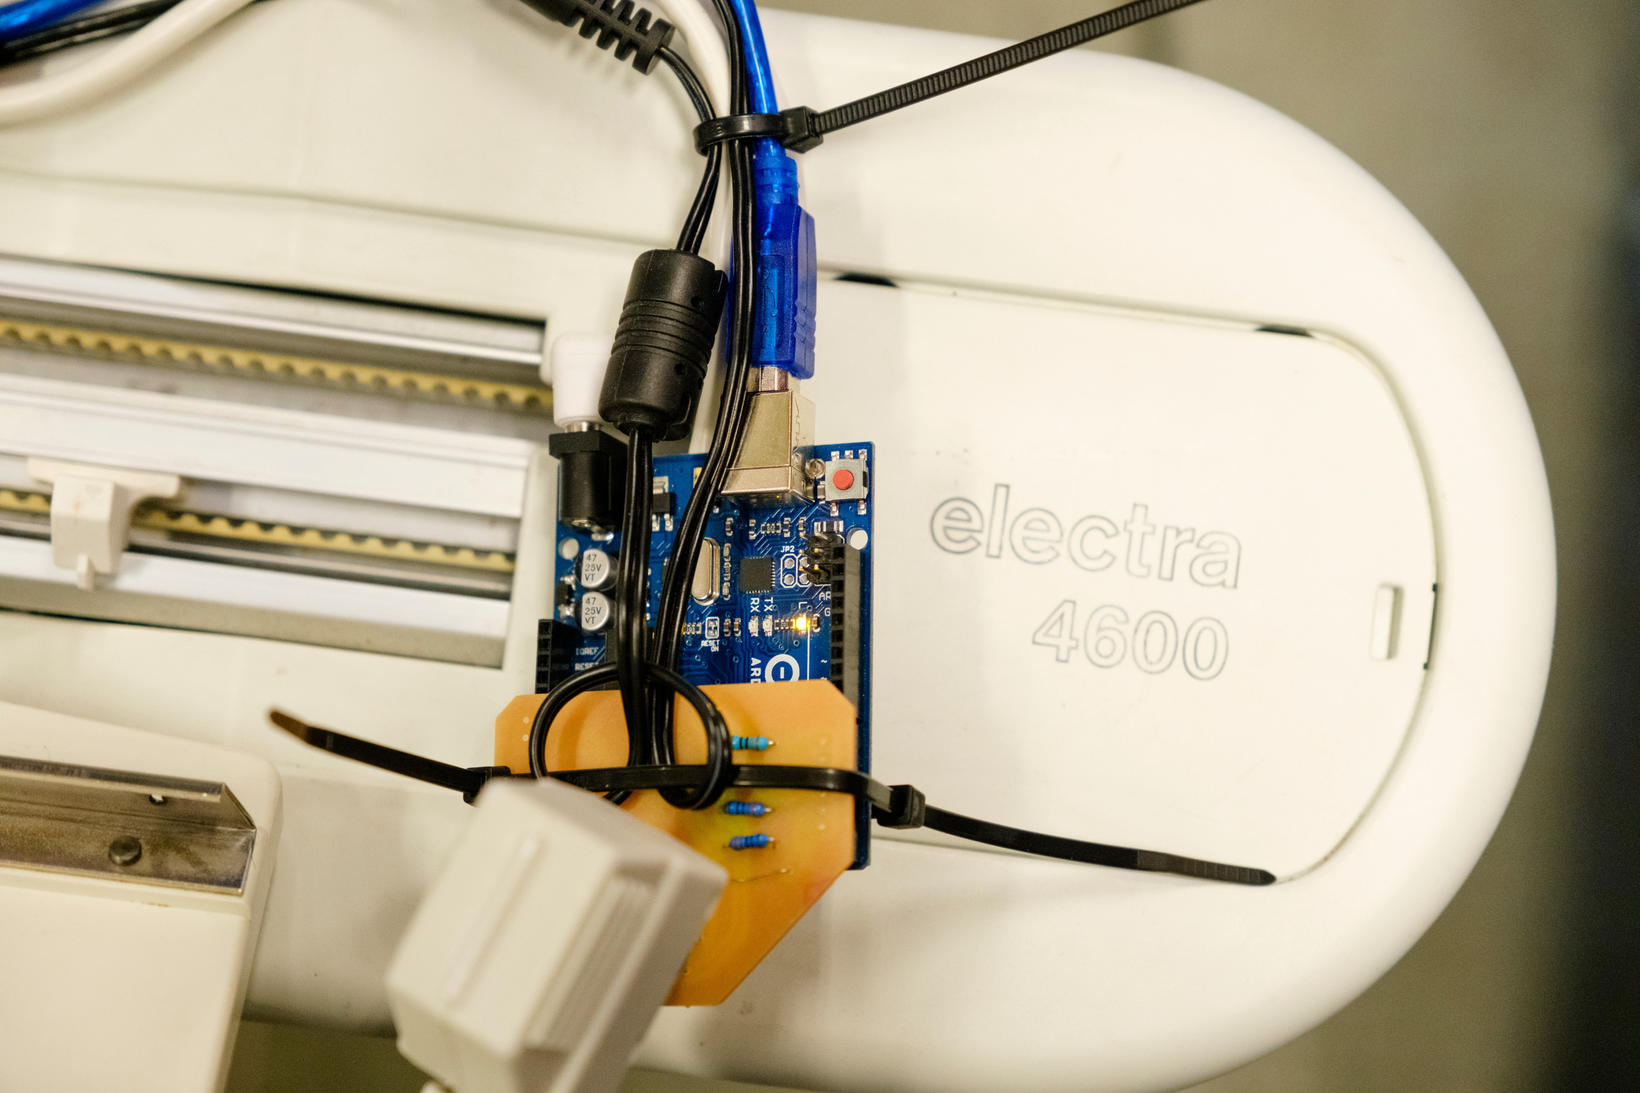
\includegraphics[width=0.8\linewidth]{figs/arduino.jpg}
    \caption{Arduino örtölva tengd við DIN-6 tengi á Passap E6000 -- \textit{mbl.is/Kristinn Magnússon}}
    \label{fig:ardino}
\end{figure}

Nýja kerfið tengist sleðanum á vélbúnaðinum beint í gegnum \emph{Arduino}, sem tekur
við merkjum frá ljósaskynjurum og stýrir nálastillurum með segulfestingum.
Skynjararnir lesa göt á braut sem sleðinn rennur eftir, og \emph{Arduino} notar þessar
upplýsingar til að ákveða hverjar nálar eigi að vera virkar í hverri umferð. 

Þessar breytingar voru innblásnar af fyrri tilraunum hackerspace-samfélaga,
sérstaklega vinnu Irene Wolf og þróunarteymis í Bamberg \cite{wolf, bamberg}.
Þeirra nálgun sýndi hvernig hægt væri að nýta eldri prjónavélar með nútímatækni og
búa til sveigjanlegt kerfi fyrir mynsturgerð og prjón.

\subsection{Sjálfvirk mynsturgerð og úrvinnsla mynsturgagna}
Hugbúnaðarhlutinn var þróaður til að umbreyta mynsturgögnum í prjónavænt snið.
Verkefnið byggir á vinnu Snæfríðar Ebbu Ásgeirsdóttur, BS nema í hagnýtri stærðfræði
og tölvunarfræði við HÍ, og felur í sér sjálfvirka aðlögun munstra fyrir vélina.

Hugbúnaðurinn inniheldur reiknirit sem umbreyta tölulegum fylkjum í prjónavænt snið.
Litir í mynstrum eru táknaðir með heiltölum og vélin getur unnið með fjóra liti í einu.
Mynstur eru unnin þannig að hver litur er prjónaður í tveimur umferðum áður en litaskipti
aðlaga prjónaröðina. Með þessum hætti er tryggt að mynstrin haldi sér vel á prjóni.

Með því að nýta gögn úr \emph{Íslensku Sjónabókinni} \cite{sjonabok} var skrifað forrit
sem umbreytir gömlum útsaumsmunstrum í stafrænt prjónamynstur. Reikniritin sem voru þróuð
skila sérsniðnum prjónamynstrum með sveigjanlegum stillingum fyrir mismunandi nálabeð.

\begin{figure}
    \centering
    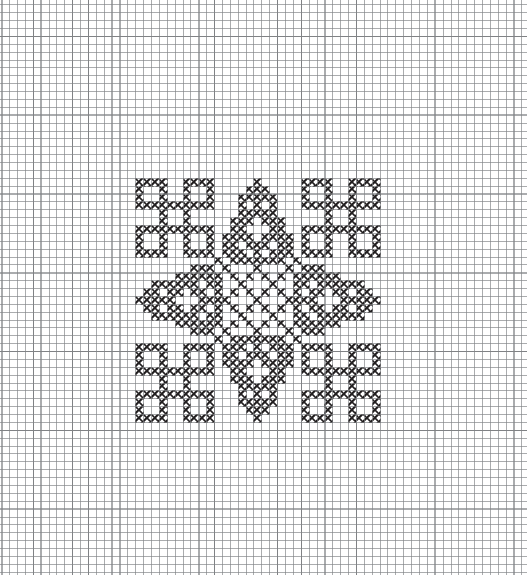
\includegraphics[height=.3\textheight]{figs/sjonabok_before.png}
    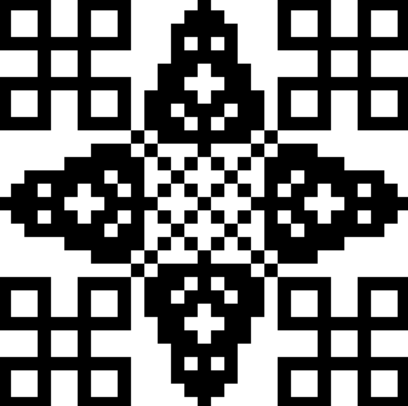
\includegraphics[height=.3\textheight]{figs/sjonabok_after.png}
    \caption{Til hægri má sjá munstur úr \textit{Íslensku Sjónabókinni} í \texttt{.eps} skrá. Til vinstri hvernig sama munstur lítur út eftir vinnslu á \texttt{.png} formi.}
    \label{fig: sjonabok_munstur}
\end{figure}


\section{Prjón og hönnunarvinna}
Fatahönnunin, sem Guðrún Ísafold Hilmarsdóttir, BA nemi í fatahönnun við LHÍ, sá um,
var órjúfanlegur hluti af verkefninu. Hún veitti fagurfræðilega leiðsögn og lagði áherslu á
hvernig útfærsla á mynstrum tengdist takmörkunum og möguleikum vélarinnar.



\begin{figure}
    \centering
    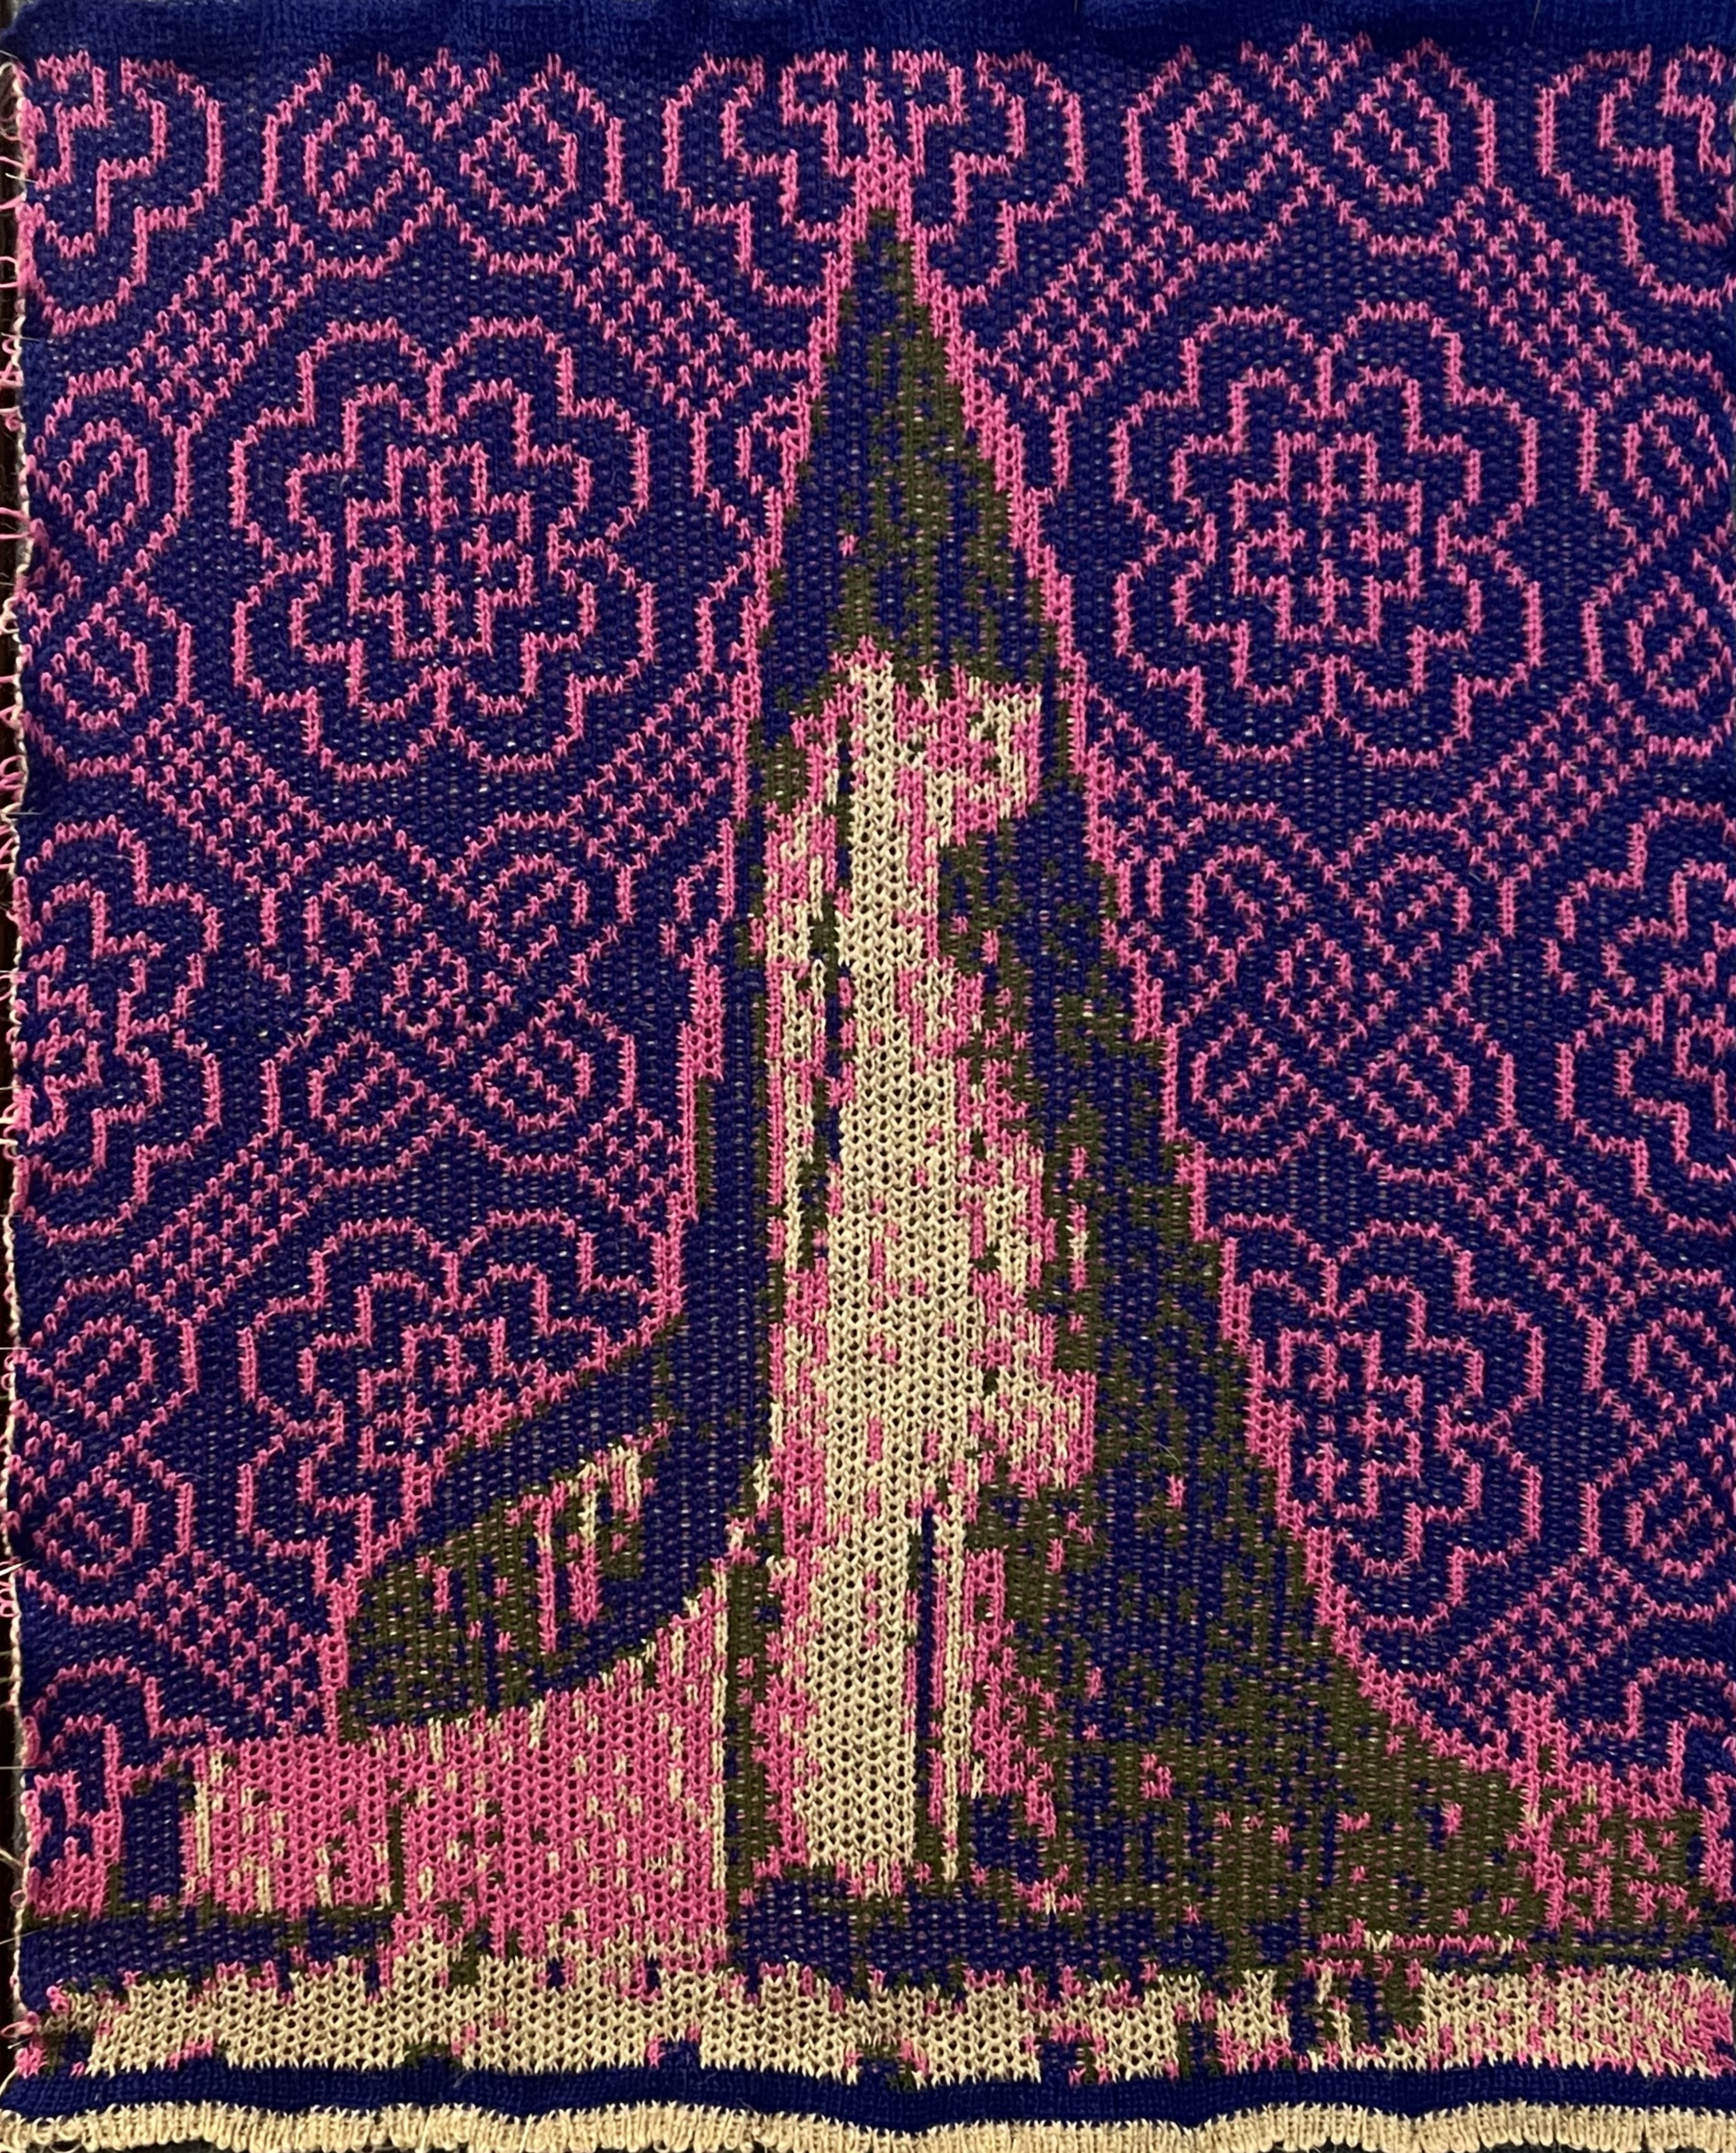
\includegraphics[width=0.5\linewidth]{figs/hallgrimskirkja.JPG}
    \caption{Hallgrímskirkja með Sjónarbókar bakgrunni}
    \label{fig:hallgrimskirkja}
\end{figure}


\begin{figure}
    \centering
    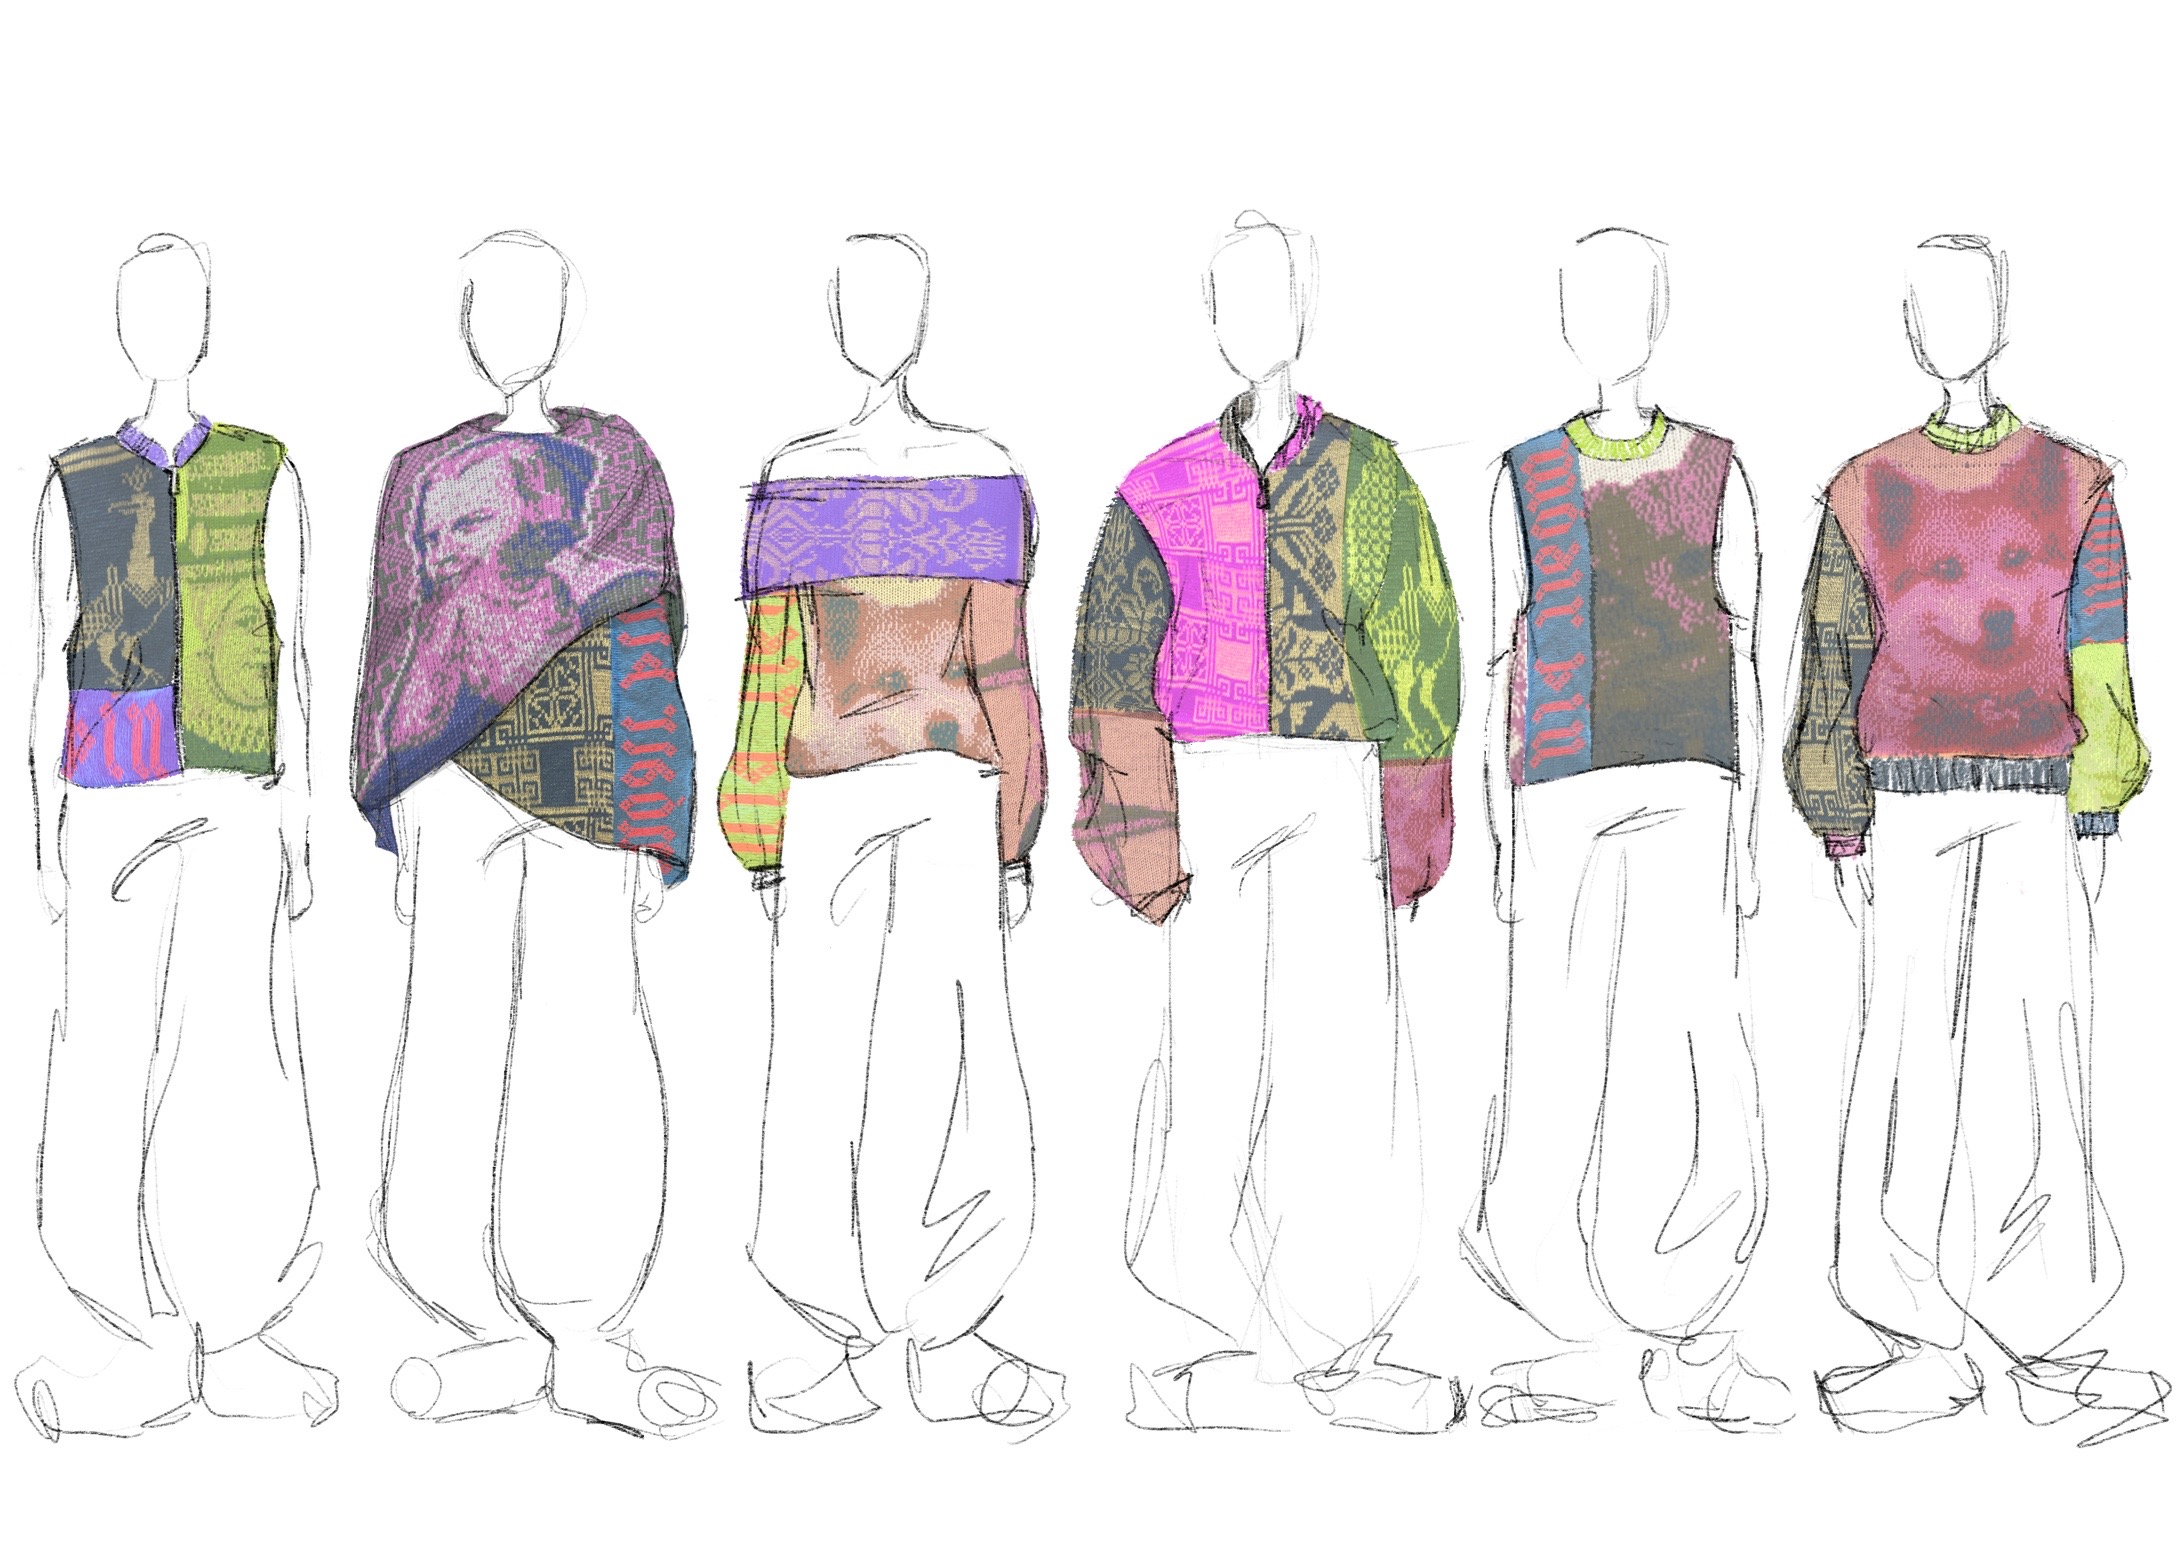
\includegraphics[width=0.8\linewidth]{figs/collection.JPG}
    \caption{Útfærslur á fatnaði út frá prjónaprufum verkefnisins.}
    \label{fig:collection}
\end{figure}



\section{Þverfaglegt samstarf}
Verkefnið sýnir hvernig samvinna milli ólíkra fræðasviða getur skapað afurð sem er
stærri en hver einstakur þátttakandi. Samstarf Guðrúnar (hönnun), Snæfríðar (hugbúnaður)
og Elíasar (vélbúnaður) tryggði að verkefnið varð heildstætt, þar sem allir þættir
tengdust í einni samþættri lausn.


\begin{figure}
    \centering
    \begin{subfigure}[b]{\textwidth}
        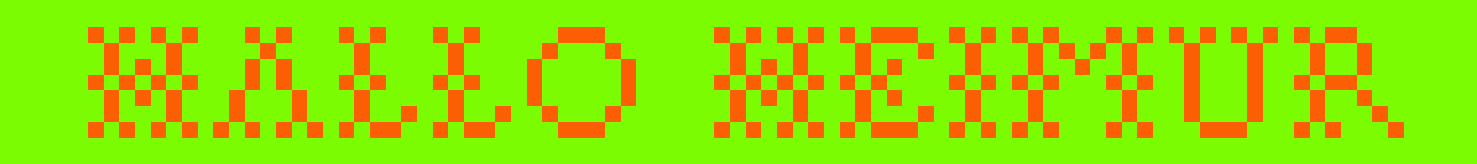
\includegraphics[width=\linewidth, clip=true, trim=0 5mm 0 0]{figs/hallo_heimur_forskrift.png}
        \caption{Forskrift}
    \end{subfigure}
    \\
    \begin{subfigure}[b]{0.48\textwidth}
        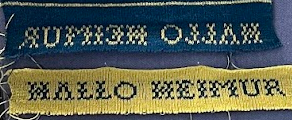
\includegraphics[width=\linewidth, clip=true, trim=0 5mm 0 0]{figs/hallo_heimur_prjon.png}
        \caption{Fyrsta atrenna}
    \end{subfigure}
    \hfill
    \begin{subfigure}[b]{0.48\textwidth}
        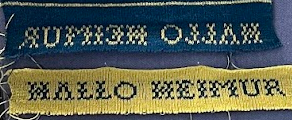
\includegraphics[width=\linewidth, clip=true, trim=0 0 0 5mm]{figs/hallo_heimur_prjon.png}
        \caption{Seinni atrenna}
    \end{subfigure}
    \caption{Þróun á prjónamynstri fyrir \textit{Halló heimur}.}
    \label{fig:hallo_heimur}
\end{figure}


\begin{figure}
    \centering
    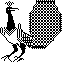
\includegraphics[height=.20\textheight]{figs/thjms5898_246_0.png}
    \hspace{24pt}
    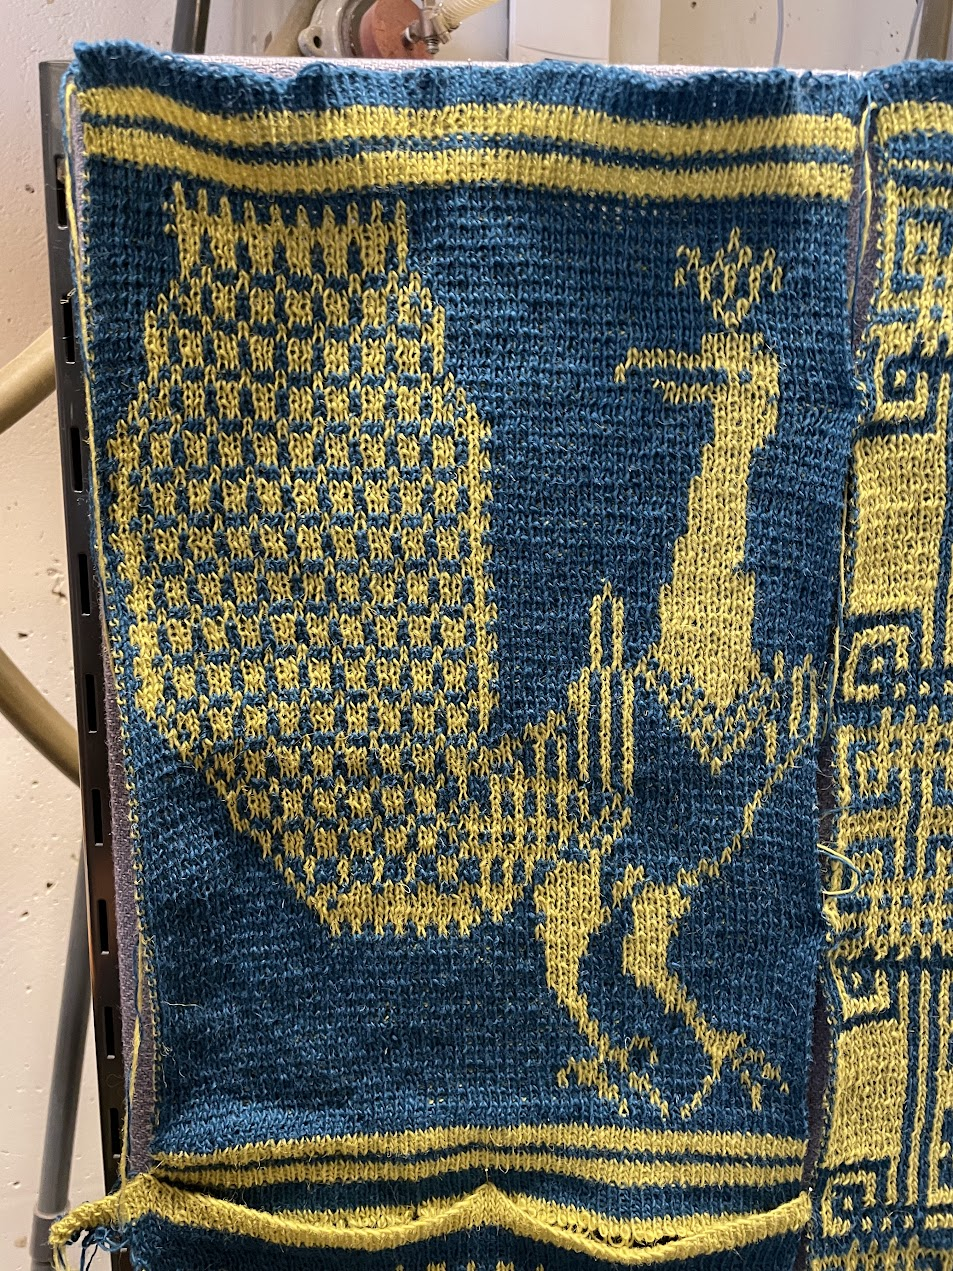
\includegraphics[height=.20\textheight]{figs/peacock.jpg}
    \caption{Páfugl, bls. 246 í Sjónabók (Þjms. 5898)}
    \label{fig:peacock}
\end{figure}

\begin{figure}
    \centering
    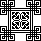
\includegraphics[height=.20\textheight]{figs/thjms5898_268.png}
    \hspace{24pt}
    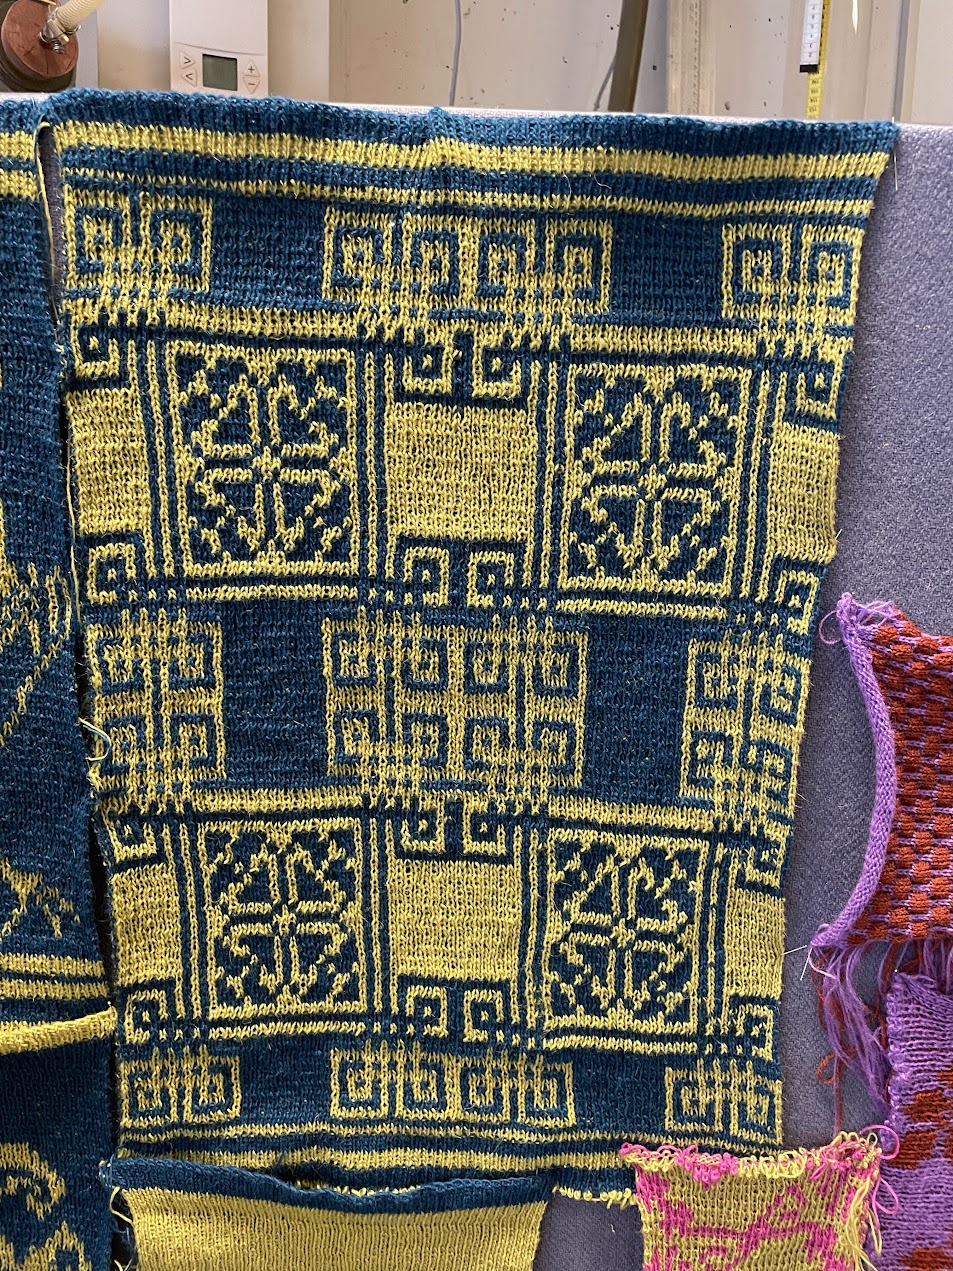
\includegraphics[height=.25\textheight]{figs/repeat.jpg}
    \caption{Endurtekið mótif, bls. 268 í Sjónabók (Þjms. 5898)}
    \label{fig:repeat}
\end{figure}

\begin{figure}
    \centering
    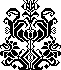
\includegraphics[height=.20\textheight]{figs/thjms5898_210.png}
    \hspace{24pt}
    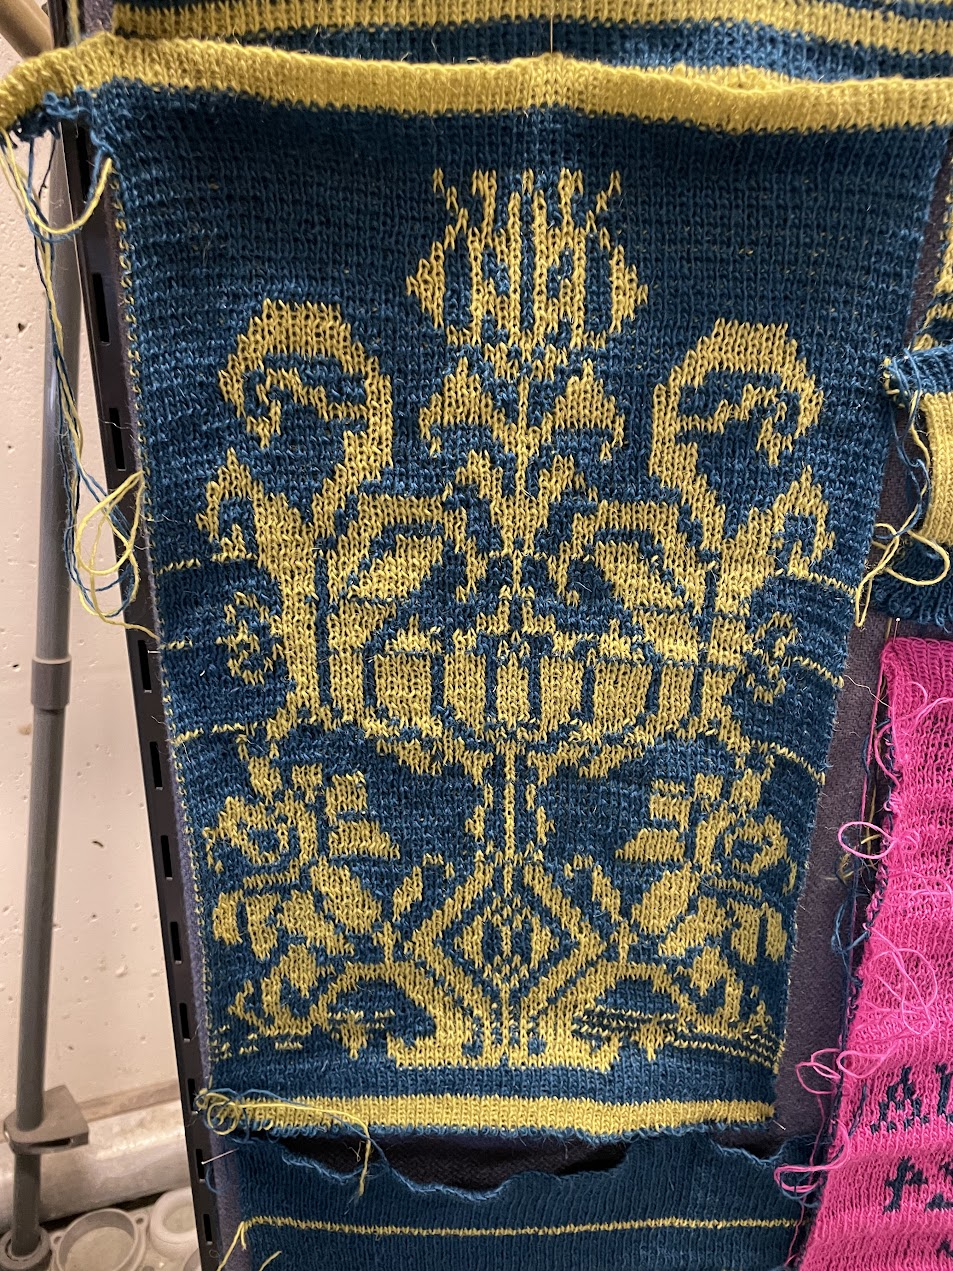
\includegraphics[height=.25\textheight]{figs/flower.jpg}
    \caption{Blóm, bls. 210 í Sjónabók (Þjms. 5898)}
    \label{fig:flower}
\end{figure}


\section{Framtíðarhorfur og næstu skref}
Næsta markmið verkefnisins er að gera vélina auðveldari til flutnings fyrir viðburði og bæta sjálfvirkni í litastýringu. 
Stefnt er að því að þróa áfram notendavænt vefviðmót sem gerir gestum og gangandi kleift að senda inn mynstur og prjóna þau í rauntíma þegar vélin er til sýnis.

Einnig er áhersla lögð á áframhaldandi samþættingu stafrænnar listsköpunar við handverk, 
þar sem prjónaferlið er nýtt sem skapandi miðill. Með þróun sjálfvirkrar mynsturgerðar og aðlögunar að sögulegum mynstrum 
er unnið að því að tengja saman forna handverkshefð og nútímatækni.

Stefnt er að sýningu á \emph{Hönnunarmars 2026}, þar sem afrakstur verkefnisins verður kynntur. Með því verður sýnt hvernig
samspil hugbúnaðar, vélbúnaðar og hönnunar getur leitt til nýrra möguleika í sjálfbærri textílframleiðslu.

Öll þróun verkefnisins er opin og aðgengileg í gegnum GitHub, \url{https://github.com/hideftextiles/}, þar sem hægt er að fylgjast með þróun hugbúnaðarins og nota hann í eigin verkefnum. 

\printbibliography

\end{document}
